\section{Resultados e Discuss\~ao}

Após a construção de modelos de determinação de idade das mangas para cada subconjunto de variáveis da Tabela \ref{tbl:var}, foram obtidas as métricas coeficiente de correlação e RMSE (Raiz do erro quadrático médio). Nos gráficos da Figura \ref{fig:metrics}, são mostrados os resultados obtidos para a \textit{Random Forest}. 

% \begin{figure}[H]
% \centering
%     \caption{Métricas obtidos para os subconjuntos de variáveis (a) Coeficiente de correlação (b) RMSE.}\label{fig:metrics}
%     \subcaptionbox{}{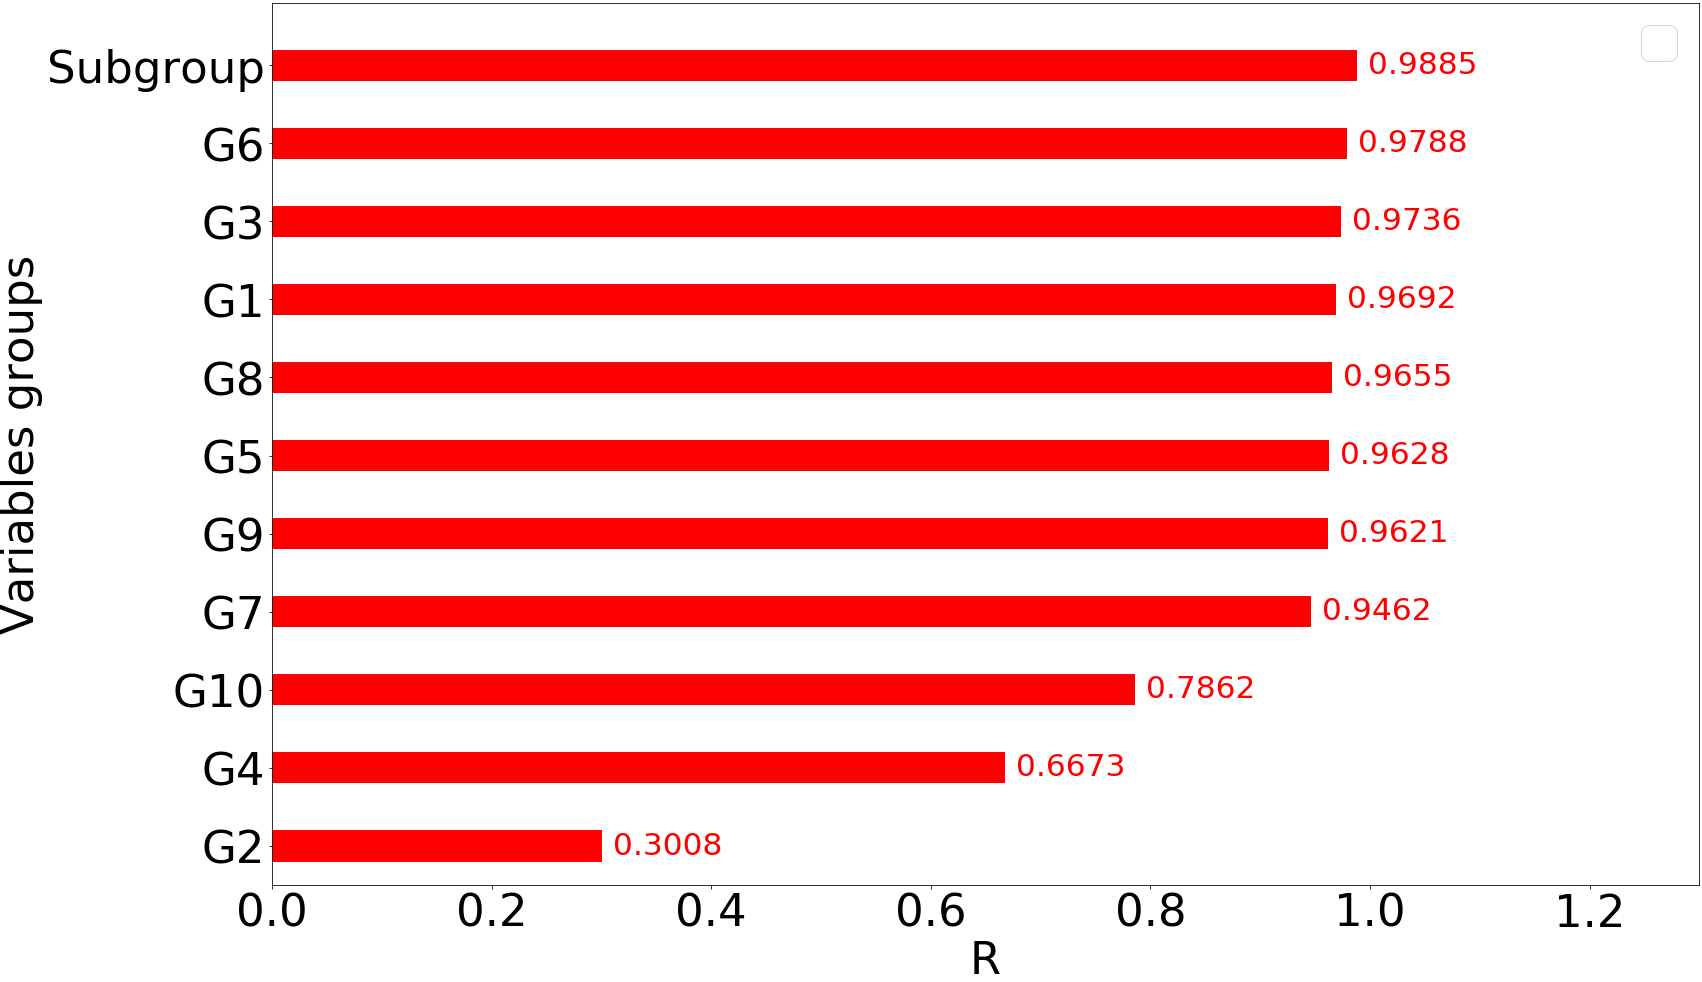
\includegraphics[scale=0.105]{imgs/results_R_subgroup.png}}
%     \subcaptionbox{}{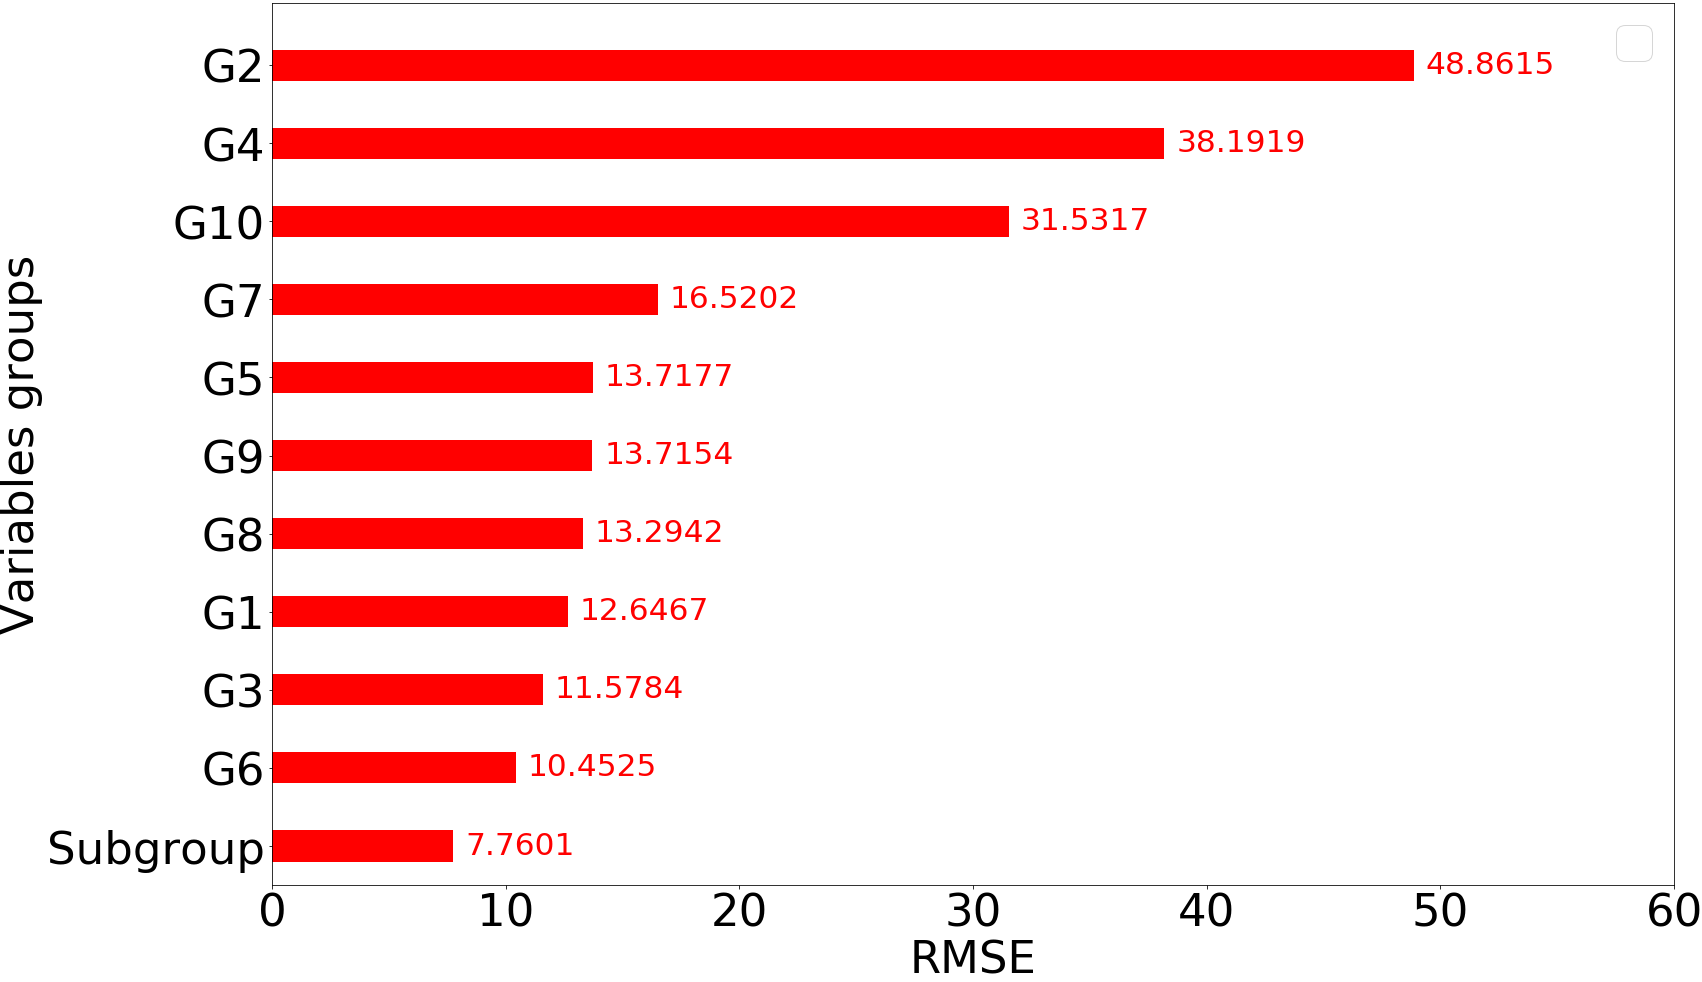
\includegraphics[scale=0.105]{imgs/results_RMSE_subgroup.png}}
% \end{figure}

\begin{figure}[H]
\centering
\begin{tabular}{rl}
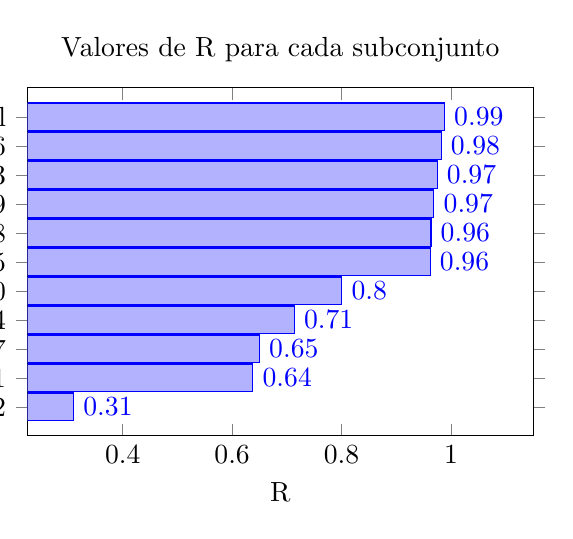
\begin{tikzpicture}[baseline,trim axis left]
    \begin{axis}[
        xbar, xmax=1.15,
        title=Valores de R para cada subconjunto,
        symbolic y coords={G2,G1,G7,G4,G10,G5,G8,G9,G3,G6,All},
        width=8cm, height=6cm,
        xlabel=R,
        ylabel=Subconjuntos,
        ytick=data,
        nodes near coords, nodes near coords align={horizontal},
        ]
        \addplot coordinates 
        {(0.988090,All)
        (0.981923,G6)
        (0.974757,G3)
        (0.968822,G9)
        (0.963391,G8)
        (0.961988,G5)
        (0.800513,G10)
        (0.713614,G4)
        (0.649978,G7)
        (0.637939,G1)
        (0.310304,G2)};
        \end{axis}
\end{tikzpicture}
&
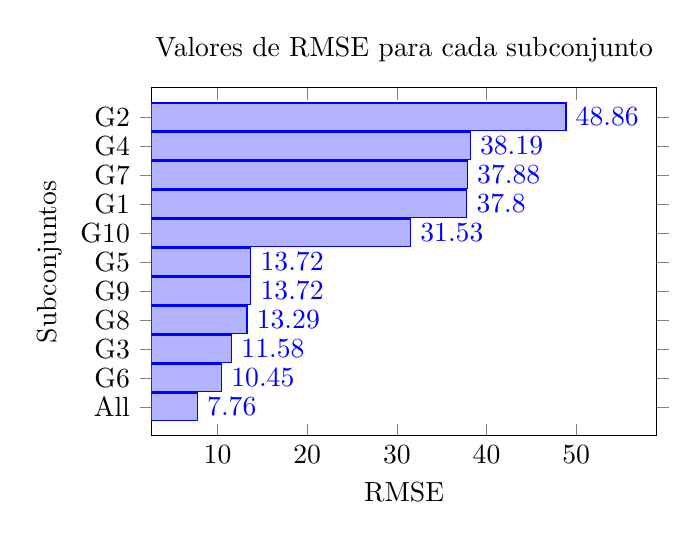
\begin{tikzpicture}[baseline,trim axis right]
    \begin{axis}[
        xbar, xmax=59,
        title=Valores de RMSE para cada subconjunto,
        symbolic y coords={All,G6,G3,G8,G9,G5,G10,G1,G7,G4,G2},
        width=8cm, height=6cm,
        xlabel=RMSE,
        ylabel=Subconjuntos,
        ytick=data,
        nodes near coords, nodes near coords align={horizontal},
        ]
        \addplot coordinates 
        {(48.861500,G2)
        (38.191900,G4)
        (37.875100,G7)
        (37.799500,G1)
        (31.531700,G10)
        (13.717700,G5)
        (13.715400,G9)
        (13.294200,G8)
        (11.578400,G3)
        (10.452500,G6)
        (7.760113,All)};
        \end{axis}
\end{tikzpicture}
\\
\end{tabular}
\caption{Métricas obtidas na determinação da idade para os subconjuntos de variáveis (a) R (b) RMSE.}\label{fig:metrics}
\end{figure}

Nota-se que os melhores resultados foram obtidos para a \textit{Random Forest} quando feita a seleção automática de variáveis. Através da técnica RFE (\textit{Random Feature Elimination}), foi obtido que as variáveis mais significantes foram as taxas R/B, R/G e S/H, média do canal B na haste, cume e equador, média do canal R na haste e cume, médias dos canais R, B, G, H e *a na manga inteira, diferença entre R e B e R e G na manga inteira, diferença entre R do cume e do equador e do cume e haste, diferença entre B do cume e haste, dimensão de correlação, área e diâmetro. Com mais informações extraídas da manga, torna-se mais provável um melhor resultado para predição da idade. Optou-se então por utilizar estas variáveis para a predição de massa, SST (Sólidos solúveis totais), firmeza e acidez titulável através da técnica \textit{ensemble}. 

\subsection{Estatística descritiva}

Após a determinação do melhor modelo para predição do tempo, foram treinadas \textit{Random Forests}, com as vinte variáveis mais significantes, para predição de massa, SST, firmeza e acidez titulável. Os modelos resultantes foram comparados aos melhores modelos da literatura. Na Tabela \ref{tbl:stats}, é mostrada a estatística descritiva dos atributos de qualidade, contendo a quantidade, média, valor mínimo e máximo, amplitude, desvio padrão e variância dos valores de referência.

\begin{table}[H]
\centering
\caption{Estatística descritiva dos valores reais de massa, SST, firmeza e acidez titulável.}\label{tbl:stats}
\begin{tabular}{llllllll}
\hline
Atributos & Amostras & M\'edia & M\'in & M\'ax & Amp & SD & Var   \\
\hline
Massa   & 1200 & 436,51  &   26,7  &   757,35  &  730,65   &  136,22   &  18557,30 \\
SST     & 1200 & 9,83    &   3,8   &   19,7    &  15,9     &  4,49     &  20,24 \\
Firmeza & 1200 & 74,048  &   2,95  &   181,4   & 178,45    & 60,80     & 3697,50 \\ 
Acidez titulável  & 1200 & 0,69    &   0,03  &   9,97    & 9,93      & 0,64      & 0,42 \\
\hline
\end{tabular}
\end{table}

Percebe-se uma grande variabilidade nos dados, o que garantiu uma maior robustez aos modelos construídos, que puderam realizar predições para mangas 'Palmer' em diferentes estágios de maturação. Nas seções posteriores são discutidos os resultados da predição de massa, SST, firmeza e acidez titulável. 

\subsection{Massa}

Com a predição de massa através da abordagem proposta e da metodologia dos autores Teoh e Syaifudin (2007), foram obtidos os valores de R e RMSE por \textit{fold}. Na Figura \ref{fig:massa_fold}, é feita uma comparação das métricas obtidas.

\begin{figure}[H]
	\centering
	\begin{tikzpicture}
	\begin{groupplot}[group style={group name = my plots, group size=2 by 2, horizontal sep = 2cm, vertical sep=2.2cm}, width = 0.5\textwidth]
	\nextgroupplot[title = R x Fold, xlabel=Fold,ylabel=R, xmin=0.8, xmax=5.2, ymin = 0.95, ymax = 1, legend style={at={(axis cs:2,0.955)}, anchor=south west}, legend cell align={left}]
	\addplot+[only marks, mark size=2pt] table[x=index, y=RF100, col sep=comma] {csv/abord_lit_massa_r.csv};
	\addlegendentry{Abordagem proposta}
	\addplot+[only marks, mark size=2pt] table[x=index, y=MLR, col sep=comma] {csv/abord_lit_massa_r.csv};
	\addlegendentry{Literatura}
	\coordinate (top) at (rel axis cs:0,1);
	\nextgroupplot[title = RMSE x Fold, xlabel=Fold,ylabel=RMSE, xmin=0.8, xmax=5.2, ymin = 12, ymax = 35, legend style={at={(axis cs:2,19)}, anchor=south west}, legend cell align={left}]
	\addplot+[only marks, mark size=2pt] table[x=index, y=RF100, col sep=comma] {csv/abord_lit_massa_rmse.csv};
	\addlegendentry{Abordagem proposta}
	\addplot+[only marks, mark size=2pt] table[x=index, y=MLR, col sep=comma] {csv/abord_lit_massa_rmse.csv};
	\addlegendentry{Literatura}
	\end{groupplot}
	\node[below=0.85cm of my plots c1r1.south]{(a)};
	\node[below=0.85cm of my plots c2r1.south]{(b)};
	
	\end{tikzpicture}
	\caption{Métricas obtidas na predição de massa de frutos da manga 'Palmer' (a) R (b) RMSE.}\label{fig:massa_fold}
\end{figure}

Nota-se que a \textit{Random Forest} foi capaz de prever massa em mangas de forma mais precisa que a Regressão linear. O coeficiente de correlação médio para a técnica \textit{ensemble} foi igual a 0,9920 e o erro médio igual a 2,98\%. Os autores Teoh e Syaifudin (2007) obtiveram, por outro lado, um coeficiente de correlação igual a 0,9769 e erro médio igual a 3,76\% para mangas da variedade Chokanan. 
Na Figura \ref{fig:scatter_massa}, são mostrados os gráficos de dispersão para o melhor modelo encontrado na literatura e para o modelo \textit{Random Forest}. Nota-se um melhor ajuste dos dados à reta para a técnica \textit{ensemble}.

\begin{figure}[H]
	\centering
	\begin{tikzpicture}
	\begin{groupplot}[group style={group name = my plots, group size=2 by 2, horizontal sep = 2cm, vertical sep=2.2cm}, width = 0.5\textwidth]
	\nextgroupplot[title = Previsto x real, xlabel=Previsto,ylabel=Real, xmin=0, xmax=800, ymin = 0, ymax = 800]
	\addplot+[only marks, mark size=0.9pt] table[col sep=comma] {csv/scatter_massa_lit.csv};
	\addplot[color=red,domain=0:800,mark=none]{0.0368 + 1*\x};
	\coordinate (top) at (rel axis cs:0,1);
	\nextgroupplot[title = Previsto x real, xlabel=Previsto,ylabel=Real, xmin=0, xmax=800, ymin = 0, ymax = 800]
	\addplot+[only marks, mark size=2pt] table[col sep=comma] {csv/scatter_massa_abord.csv};
	\addplot[color=red,domain=0:800,mark=none]{-1.63 + 1*\x};
	\end{groupplot}
	\node[below=0.85cm of my plots c1r1.south]{(a)};
	\node[below=0.85cm of my plots c2r1.south]{(b)};
	
	\end{tikzpicture}
	\caption{Gráficos de dispersão para massa (a) Modelo da literatura (b) Abordagem proposta.}\label{fig:scatter_massa}
\end{figure}

\color{red}Na Tabela \ref{tbl:hip_massa}, é feito um resumo dos testes de hipótese para massa. \color{black}

\begin{table}[H]
    \centering
    \caption{Resumo dos testes de hipótese para massa.}
    \begin{tabular}{ccccc}
        \hline
         \textbf{Métrica} & $\mu1$ & $\mu2$ & $\mu1 - \mu2$ & $p$-value \\ \hline
         RMSE & 16.9961 & 29.8469   & -12.8507  & \\ 
         R    & 0.9919  & 0.9754    & 0.0165    & \\ \hline
    \end{tabular}
    \label{tbl:hip_massa}
\end{table}

% A partir da propriedade do modelo RF construído, é possível obter as variáveis de entrada mais significantes para predição do atributo alvo. Na Figura \ref{fig:massa_imp}, são mostradas as três variáveis mais importantes para determinação da massa em mangas 'Palmer'. Nota-se que a variável calculada pelos autores Teoh e Sayfudin (2007) não foi a mais significativa para prever a massa em mangas. A dimensão de correlação, variável fractal que avalia a complexidade de um sistema (MCMAHON; TOOMEY; KANE, 2017), foi a mais significante para o modelo, seguida pelo diâmetro estimado e, por fim, o número de pixels que correspondem à manga. 

% \begin{figure}[H]
% \centering
%     \caption{Variáveis mais importantes do modelo RF para predição da massa.}\label{fig:massa_imp}
%     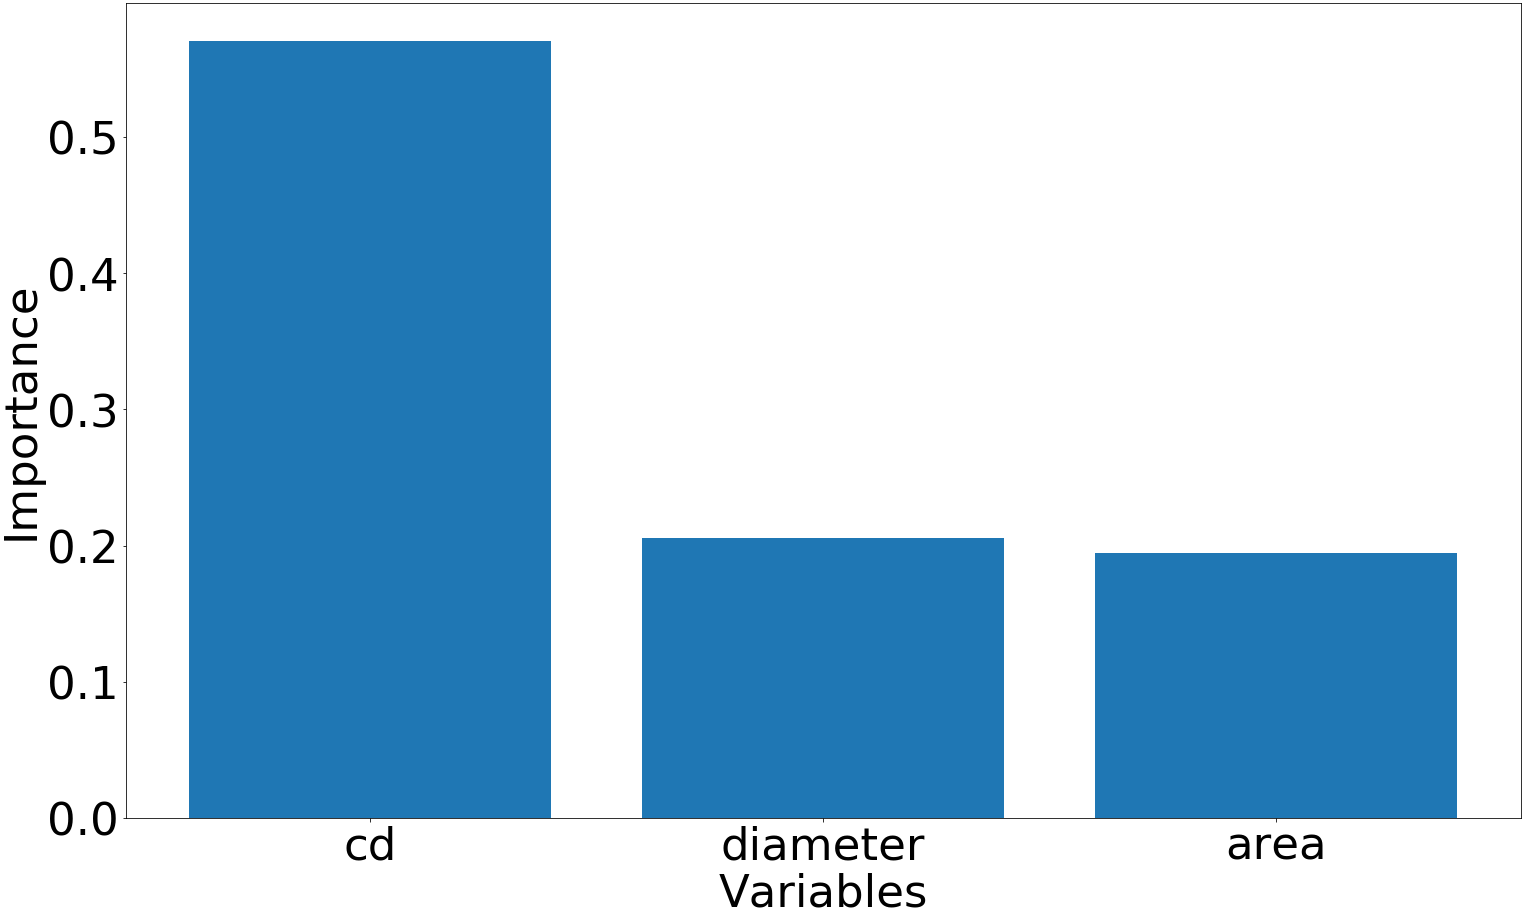
\includegraphics[scale=0.15]{imgs/importancia_massa.png}
% \end{figure}

\subsection{Sólidos solúveis totais (SST)}

Ao empregar a metodologia de Khairunniza-Bejo e Kamarudin (2011) para predição de SST, foi obtido um coeficiente de correlação médio inferior a 0.1 e RMSE médio igual a 4.48, enquanto que os autores alcançaram valores iguais a -0,92 e 0,033 ºBrix respectivamente para mangas da variedade Chokanan.

Nota-se que para a variedade 'Palmer', um modelo linear que emprega apenas uma variável, a matiz, é insuficiente para a determinação precisa de SST. Por outro lado, ao empregar a abordagem proposta, foram obtidos valores médios de R e RMSE iguais a 0,9797 e 0,8946 ºBrix. Na Figura \ref{fig:sst_fold}, são mostradas as métricas por \textit{fold} para a Regressão linear e \textit{Random Forest}.

\begin{figure}[H]
	\centering
	\begin{tikzpicture}
    	\begin{groupplot}[group style={group name = my plots, group size=2 by 2, horizontal sep = 2cm, vertical sep=2.2cm}, width = 0.5\textwidth]
        	\nextgroupplot[title = R x Fold, xlabel=Fold,ylabel=R, xmin=0.8, xmax=5.2, ymin=0, ymax=1.1, legend style={at={(axis cs:2,0.4)}, anchor=south west}, legend cell align={left}]
        	\addplot+[only marks, mark size=2pt] table[x=index, y=RF100, col sep=comma] {csv/abord_lit_sst_r.csv};
        	\addlegendentry{Abordagem proposta}
        	\addplot+[only marks, mark size=2pt] table[x=index, y=MLR, col sep=comma] {csv/abord_lit_sst_r.csv};
        	\addlegendentry{Literatura}
        	\coordinate (top) at (rel axis cs:0,1);
        	\nextgroupplot[title = RMSE x Fold, xlabel=Fold,ylabel=RMSE, xmin=0.8, xmax=5.2, ymin = 0, ymax=5, legend style={at={(axis cs:2,2)}, anchor=south west}, legend cell align={left}]
        	\addplot+[only marks, mark size=2pt] table[x=index, y=RF100, col sep=comma] {csv/abord_lit_sst_rmse.csv};
        	\addlegendentry{Abordagem proposta}
        	\addplot+[only marks, mark size=2pt] table[x=index, y=MLR, col sep=comma] {csv/abord_lit_sst_rmse.csv};
        	\addlegendentry{Literatura}
    	\end{groupplot}
    	\node[below=0.85cm of my plots c1r1.south]{(a)};
    	\node[below=0.85cm of my plots c2r1.south]{(b)};
	\end{tikzpicture}
	\caption{Métricas obtidas na predição de SST de frutos da manga 'Palmer' (a) R (b) RMSE.}\label{fig:sst_fold}
\end{figure}

Assim, o valor de R obtido no presente estudo foi superior aos encontrados na literatura. Por outro lado, o RMSE ainda foi maior que o obtido por Khairunniza-Bejo e Kamarudin (2011).

Na Figura \ref{fig:scatter_sst}, são mostrados os gráficos de dispersão para a Regressão linear com a matiz de entrada e para o modelo \textit{Random Forest} com as melhores variáveis.

\begin{figure}[H]
    \centering
    \begin{tikzpicture}
    \begin{groupplot}[group style={group name = my plots, group size=2 by 2, horizontal sep = 2cm, vertical sep=2.2cm}, width = 0.5\textwidth]
    \nextgroupplot[title = Previsto x real, xlabel=Previsto,ylabel=Real, xmin=0, xmax=20, ymin = 0, ymax = 20]
    \addplot+[only marks, mark size=1pt] table[col sep=comma] {csv/scatter_sst_lit.csv};
    \addplot[color=red,domain=0:20,mark=none]{3.53 + 0.641*\x};
    \coordinate (top) at (rel axis cs:0,1);
    \nextgroupplot[title = Previsto x real, xlabel=Previsto,ylabel=Real, xmin=0, xmax=20, ymin = 0, ymax = 20]
    \addplot+[only marks, mark size=1pt] table[col sep=comma] {csv/scatter_sst_abord.csv};
    \addplot[color=red,domain=0:20,mark=none]{-0.168 + 1.01*\x};
    \end{groupplot}
    \node[below=0.85cm of my plots c1r1.south]{(a)};
    \node[below=0.85cm of my plots c2r1.south]{(b)};
    \end{tikzpicture}
    \caption{Gráficos de dispersão para SST (a) Modelo da literatura (b) Abordagem proposta.}\label{fig:scatter_sst}
\end{figure}

Mais uma vez foi obtido um melhor ajuste dos dados para a técnica \textit{ensemble}. Por possuir mais informações da manga como entrada do modelo, o relacionamento com o SST foi modelado de forma mais precisa.

\color{red}Na Tabela \ref{tbl:hip_sst}, é feito um resumo dos testes de hipótese para SST. \color{black}

\begin{table}[H]
    \centering
    \caption{Resumo dos testes de hipótese para SST.}
    \begin{tabular}{ccccc}
        \hline
         \textbf{Métrica} & $\mu1$ & $\mu2$ & $\mu1 - \mu2$ & $p$-value \\ \hline
         RMSE & 0.8988 & 4.4790   & -3.5802  & \\ 
         R    & 0.9793 & 0.0890    & 0.8902  & \\ \hline
    \end{tabular}
    \label{tbl:hip_sst}
\end{table}


% Na predição de SST pela \textit{Random Forest}, foi encontrado que as variáveis mais significantes foram a taxa R/B, dimensão de correlação e média do canal B na região equatorial da manga, conforme mostra a Figura \ref{fig:sst_imp}.

% \begin{figure}[H]
% \centering
%     \caption{Variáveis mais importantes do modelo RF para predição da SST.}\label{fig:sst_imp}
%     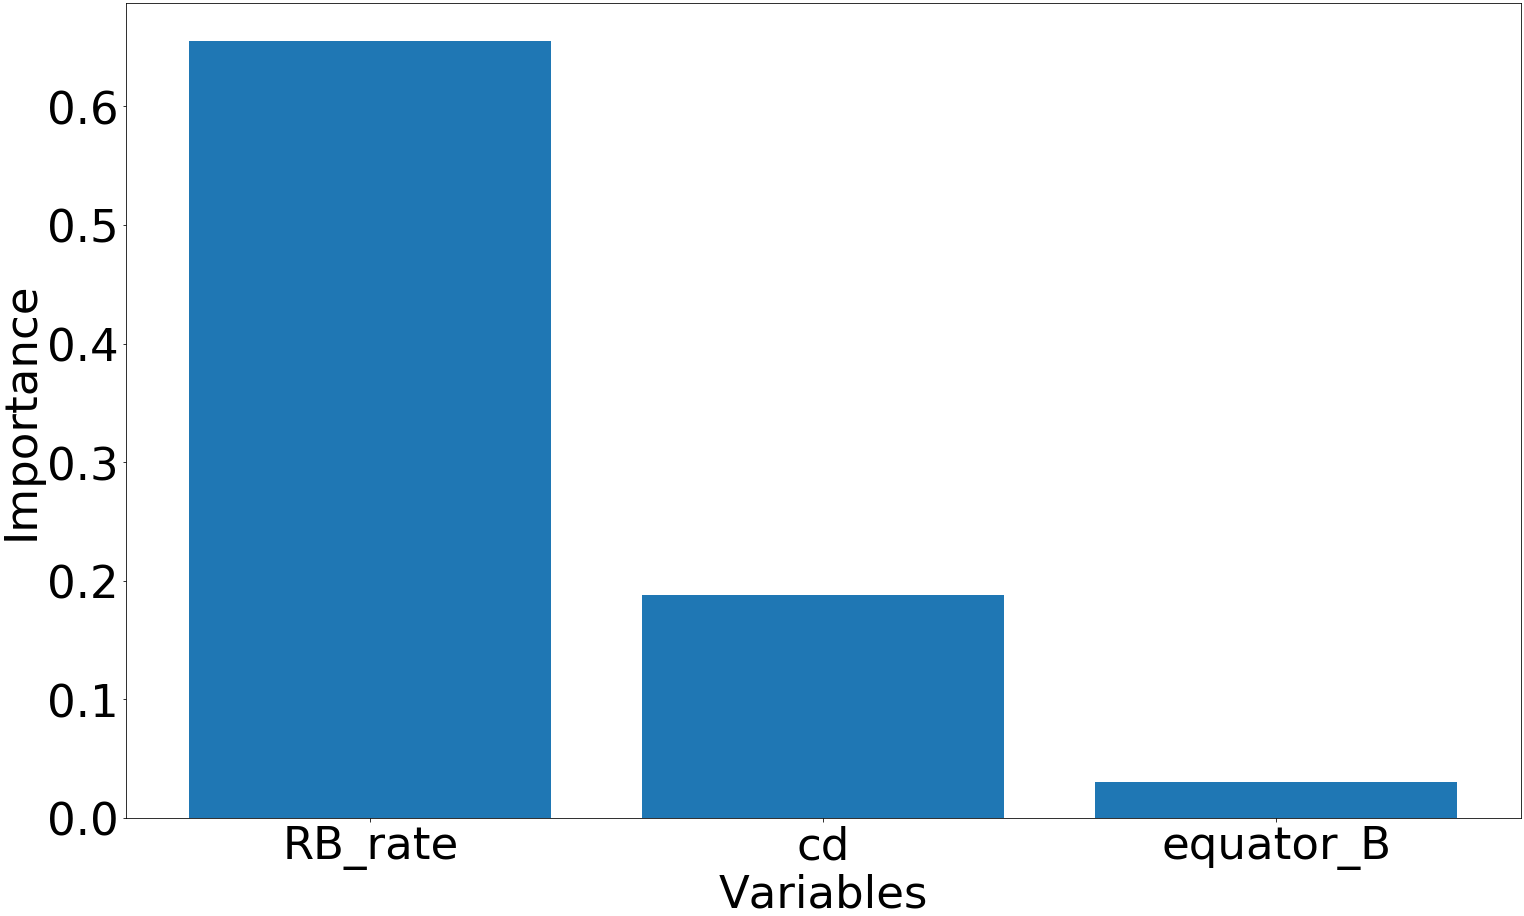
\includegraphics[scale=0.15]{imgs/importancia_sst.png}
% \end{figure}

% Enquanto os autores Khairunniza-Bejo e Kamarudin (2011) encontraram bons resultados utilizando o espaço de cores HSV, para a variedade 'Palmer' nota-se que o espaço RGB foi o mais significante. O atributo mais importante consistiu na taxa R/B, em que R e B são, respectivamente, os valores médios dos pixels no canal R e B. Ademais, a média no espaço B para região equatorial da manga, que consiste em sua região central, também foi importante para o modelo. Por fim, a dimensão de correlação mostrou-se determinante para o SST da mesma forma que foi para a massa.

\subsection{Firmeza}

Ao empregar o valor médio dos pixels no canal L* como entrada em uma Regressão linear, foi obtido um valor médio de R igual a 0,1860, muito menor que o obtido por Abarra et al. (2018), que obtiveram um coeficiente igual a 0,968. Assim, nota-se que essa variável não varia linearmente para a variedade 'Palmer', diferentemente da variedade empregada pelos autores, a Carabao.

Por outro lado, através do modelo \textit{Random Forest}, que emprega as vinte variáveis mais significantes, foi alcançado um coeficiente de correlação médio igual a 0,9674, ainda menor que o obtido pelos autores, mas bastante maior que o obtido anteriormente. Os valores de R e RMSE por \textit{fold} são mostrados na Figura \ref{fig:firm_fold}.

\begin{figure}[H]
	\centering
	\begin{tikzpicture}
    	\begin{groupplot}[group style={group name = my plots, group size=2 by 2, horizontal sep = 2cm, vertical sep=2.2cm}, width = 0.5\textwidth]
        	\nextgroupplot[title = R x Fold, xlabel=Fold,ylabel=R, xmin=0.8, xmax=5.2, ymin = -0.1, ymax = 1.1, legend style={at={(axis cs:2,0.4)},anchor=south west}, legend cell align={left}]
        	\addplot+[only marks, mark size=2pt] table[x=index, y=RF100, col sep=comma] {csv/abord_lit_firmeza_r.csv};
        	\addlegendentry{Abordagem proposta}
        	\addplot+[only marks, mark size=2pt] table[x=index, y=MLR, col sep=comma] {csv/abord_lit_firmeza_r.csv};
        	\addlegendentry{Literatura}
        	\coordinate (top) at (rel axis cs:0,1);
        	\nextgroupplot[title = RMSE x Fold, xlabel=Fold,ylabel=RMSE, xmin=0.8, xmax=5.2, ymin = 10, ymax = 65, legend style={at={(axis cs:2,32)}, anchor=south west}, legend cell align={left}]
        	\addplot+[only marks, mark size=2pt] table[x=index, y=RF100, col sep=comma] {csv/abord_lit_firmeza_rmse.csv};
        	\addlegendentry{Abordagem proposta}
        	\addplot+[only marks, mark size=2pt] table[x=index, y=MLR, col sep=comma] {csv/abord_lit_firmeza_rmse.csv};
        	\addlegendentry{Literatura}
    	\end{groupplot}
    	\node[below=0.85cm of my plots c1r1.south]{(a)};
    	\node[below=0.85cm of my plots c2r1.south]{(b)};
	\end{tikzpicture}
	\caption{Métricas obtidas na predição de firmeza de frutos da manga 'Palmer' (a) R (b) RMSE.}\label{fig:firm_fold}
\end{figure}

Na Figura \ref{fig:scatter_firmeza}, são mostrados os gráficos de dispersão para os dois modelos de predição de firmeza. Nota-se um ajuste muito pobre para o modelo linear, enquanto que no modelo não linear os dados concentram-se mais ao redor da reta. 

\begin{figure}[H]
	\centering
	\begin{tikzpicture}
	\begin{groupplot}[group style={group name = my plots, group size=2 by 2, horizontal sep = 2cm, vertical sep=2.2cm}, width = 0.5\textwidth]
	\nextgroupplot[title = Previsto x real, xlabel=Previsto,ylabel=Real, xmin=0, xmax=175, ymin = 0, ymax = 175]
	\addplot+[only marks, mark size=1pt] table[col sep=comma] {csv/scatter_firmeza_lit.csv};
	\addplot[color=red,domain=0:175,mark=none]{375 - 4.06*\x};
	\coordinate (top) at (rel axis cs:0,1);
	\nextgroupplot[title = Previsto x real, xlabel=Previsto,ylabel=Real, xmin=0, xmax=175, ymin = 0, ymax = 175]
	\addplot+[only marks, mark size=1pt] table[col sep=comma] {csv/scatter_firmeza_abord.csv};
	\addplot[color=red,domain=0:175,mark=none]{0.121 + 1.01*\x};
	\end{groupplot}
	\node[below=0.85cm of my plots c1r1.south]{(a)};
	\node[below=0.85cm of my plots c2r1.south]{(b)};
	
	\end{tikzpicture}
	\caption{Gráficos de dispersão para firmeza (a) Modelo da literatura (b) Abordagem proposta.}\label{fig:scatter_firmeza}
\end{figure}

\color{red}Na Tabela \ref{tbl:hip_firm}, é feito um resumo dos testes de hipótese para firmeza. \color{black}

\begin{table}[H]
    \centering
    \caption{Resumo dos testes de hipótese para firmeza.}
    \begin{tabular}{ccccc}
        \hline
         \textbf{Métrica} & $\mu1$ & $\mu2$ & $\mu1 - \mu2$ & $p$-value \\ \hline
         RMSE & 15.2894 & 60.8198  & -45.5303   & \\ 
         R    & 0.9674  & 0.04516  & 0.9222     & \\ \hline
    \end{tabular}
    \label{tbl:hip_firm}
\end{table}

% Por fim, são mostradas na Figura \ref{fig:firm_imp} as variáveis mais significantes para o modelo RF na determinação da firmeza.

% \begin{figure}[H]
% \centering
%     \caption{Variáveis mais importantes do modelo RF para predição da firmeza.}\label{fig:firm_imp}
%     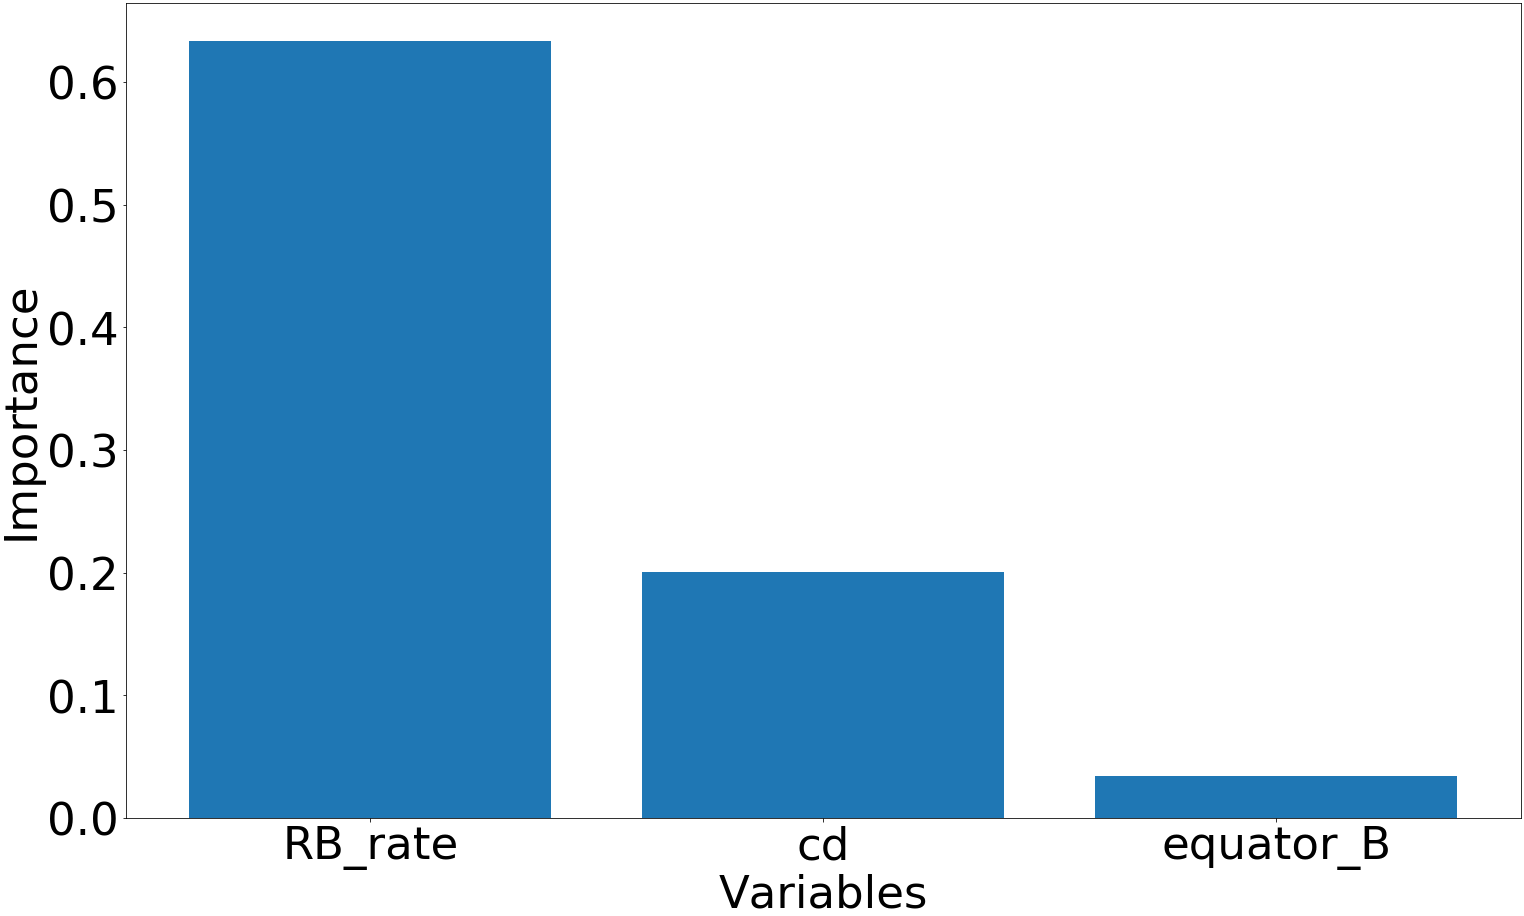
\includegraphics[scale=0.15]{imgs/importancia_firmeza.png}
% \end{figure}

% Percebe-se que os três atributos mais importantes para o modelo de predição de firmeza são os mesmos vistos para o SST, como visto na Figura \ref{fig:sst_imp}. O valor da importância de cada variável mostrou-se bastante similar da mesma forma.

\subsection{Acidez titulável}
Da mesma forma que para a firmeza, foi utilizada a variável L* como entrada em um modelo linear. Enquanto que os autores Abarra et al. (2018) alcançaram um coeficiente de correlação igual a 0,977 para a variedade Carabao, foi obtido um valor de R igual a 0,3882 para a 'Palmer'. Neste caso, também, o atributo Acidez titulável não possui uma relação linear com a variável L*.

Ao empregar a \textit{Random Forest}, foram obtidos resultados significativamente maiores, com um valor médio de R igual a 0,9077, mas ainda menor que o obtido pelos autores. 

As métricas para ambos modelos são mostrados na Figura \ref{fig:acdz_fold}.

\begin{figure}[H]
	\centering
	\begin{tikzpicture}
	\begin{groupplot}[group style={group name = my plots, group size=2 by 2, horizontal sep = 2cm, vertical sep=2.2cm}, width = 0.5\textwidth]
    	\nextgroupplot[title = R x Fold, xlabel=Fold,ylabel=R, xmin=0.8, xmax=5.2, ymin = 0, ymax = 1.1, legend style={at={(axis cs:2,0.03)}, anchor=south west}, legend cell align={left}]
    	\addplot+[only marks, mark size=2pt] table[x=index, y=RF100, col sep=comma] {csv/abord_lit_acidez_r.csv};
    	\addlegendentry{Abordagem proposta}
    	\addplot+[only marks, mark size=2pt] table[x=index, y=MLR, col sep=comma] {csv/abord_lit_acidez_r.csv};
    	\addlegendentry{Literatura}
    	\coordinate (top) at (rel axis cs:0,1);
    	\nextgroupplot[title = RMSE x Fold, xlabel=Fold,ylabel=RMSE, xmin=0.8, xmax=5.2, ymin = 0.1, ymax = 1, legend style={at={(axis cs:2,0.77)}, anchor=south west}, legend cell align={left}]
    	\addplot+[only marks, mark size=2pt] table[x=index, y=RF100, col sep=comma] {csv/abord_lit_acidez_rmse.csv};
    	\addlegendentry{Abordagem proposta}
    	\addplot+[only marks, mark size=2pt] table[x=index, y=MLR, col sep=comma] {csv/abord_lit_acidez_rmse.csv};
    	\addlegendentry{Literatura}
	\end{groupplot}
	\node[below=0.85cm of my plots c1r1.south]{(a)};
	\node[below=0.85cm of my plots c2r1.south]{(b)};
	\end{tikzpicture}
	\caption{Métricas obtidas na predição de acidez titulável de frutos da manga 'Palmer' (a) R (b) RMSE.}\label{fig:acdz_fold}
\end{figure}

Na Figura \ref{fig:scatter_acidez}, são mostrados os gráficos de dispersão para os dois modelos de predição de acidez titulável. O modelo proposto é claramente superior ao sugerido para a literatura, mas ainda sim inferior ao obtido pelos autores. Nota-se que, assim como para a firmeza, a relação da acidez titulável com o valor médio de L* não é linear. Isto pode ser explicado pelo fato de que as mangas utilizadas pelos autores eram da variedade Carabao, e não 'Palmer'. 

\begin{figure}[H]
	\centering
	\begin{tikzpicture}
	\begin{groupplot}[group style={group name = my plots, group size=2 by 2, horizontal sep = 2cm, vertical sep=2.2cm}, width = 0.5\textwidth]
	\nextgroupplot[title = Previsto x real, xlabel=Previsto,ylabel=Real, xmin=0, xmax=2, ymin = 0, ymax = 2]
	\addplot+[only marks, mark size=1pt] table[col sep=comma] {csv/scatter_acidez_lit.csv};
	\addplot[color=red,mark=none]{0.0101 + 0.985*\x};
	\coordinate (top) at (rel axis cs:0,1);
	\nextgroupplot[title = Previsto x real, xlabel=Previsto,ylabel=Real, xmin=0, xmax=2, ymin = 0, ymax = 2]
	\addplot+[only marks, mark size=1pt] table[col sep=comma] {csv/scatter_acidez_abord.csv};
	\addplot[color=red,mark=none]{0.0129 + 0.98*\x};
	\end{groupplot}
	\node[below=0.85cm of my plots c1r1.south]{(a)};
	\node[below=0.85cm of my plots c2r1.south]{(b)};
	\end{tikzpicture}
	\caption{Gráficos de dispersão para acidez titulável (a) Modelo da literatura (b) Abordagem proposta.}\label{fig:scatter_acidez}
\end{figure}

\color{red}Na Tabela \ref{tbl:hip_acdz}, é feito um resumo dos testes de hipótese para acidez titulável. \color{black}

\begin{table}[H]
    \centering
    \caption{Resumo dos testes de hipótese para acidez titulável.}
    \begin{tabular}{ccccc}
        \hline
         \textbf{Métrica} & $\mu1$ & $\mu2$ & $\mu1 - \mu2$ & $p$-value \\ \hline
         RMSE & 0.2624 & 0.5894  & -0.3270   & \\ 
         R    & 0.9023 & 0.3882  & 0.5140    & \\ \hline
    \end{tabular}
    \label{tbl:hip_acdz}
\end{table}